\begin{minipage}{10 cm}{
\Large
\textit{   Un ni�ito le dijo a su amigo: ``Mira yo le ense�� a mi perro Tobi a silbar''. El otro ni�o puso su oreja junto a la trompa del perro y dijo:``Yo no lo oigo silba''. El peque�o profesor respondi�:``Yo dije que le ense��, no dije que aprendi�.''} \normalsize An�nimo...
}
\end{minipage}
\begin{minipage}{6 cm}{
\begin{center}
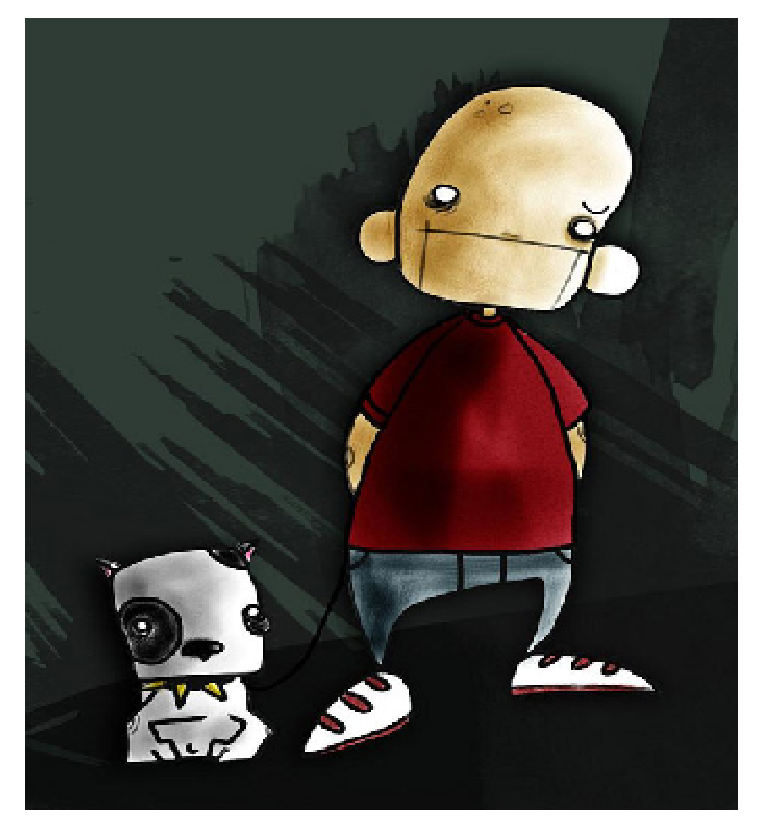
\includegraphics[scale=0.4]{a-fig1}
%\caption{Tobi y su perro}
\end{center}
}
\end{minipage}

\section*{�Qu� pas� con Tobi?}
\begin{itemize}
\item Es posible que el peque�o profesor no haya aplicado la metodolog�a adecuada
\item Otra hip�tesis es que Tobi no posea la capacidad para aprender a silbar
\item Una tercera hip�tesis, es que a Tobi no le interesa aprender a silbar
\end{itemize}

\section*{An�lisis de este caso}
\begin{itemize}
\item El inter�s y la necesidad de aprender algo, tienen que nacer de adentro
\item La funci�n del profesor, es estimular que se genere esa necesidad y facilitar que esa necesidad pueda satisfacerse 
\end{itemize}

\section*{Conclusiones}
\begin{itemize}
\item Nadie puede aprender por otros, el inter�s por el aprendizaje debe generarse en el interior de la persona
\item Las materias no tiene una existencia real aunque est�n escritas en los libros, lo que existe son las personas y sus problemas, por tanto es menos importante almacenar informaci�n y es mas importante el inter�s por aprender
\item Las personas aprenden lo que les interesa
\end{itemize}